%********************************************************************
% Appendix
%*******************************************************
% If problems with the headers: get headings in appendix etc. right
%\markboth{\spacedlowsmallcaps{Appendix}}{\spacedlowsmallcaps{Appendix}}
\chapter{Appendix to AtomicOrchid implementation}


\section{System architecture}
\begin{figure}[H]
  \centering
  \rotatebox{90}{
  	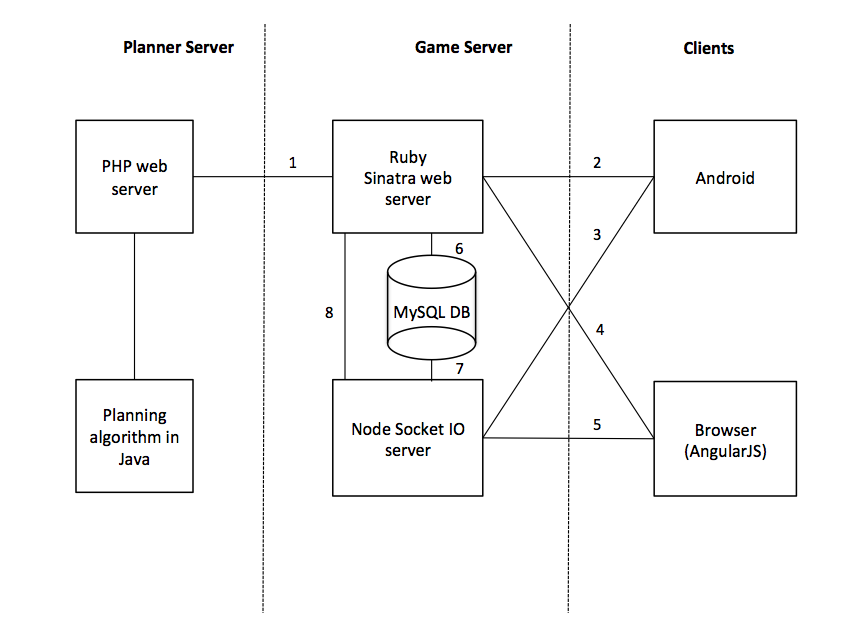
\includegraphics[width=1.2\textwidth]{img/Appendix/SystemDescription}
  }
  \caption{Technological illustration of AtomicOrchid}
  \label{fig:systemDescription}
\end{figure}

\begin{table}[H]
\centering
\footnotesize
\begin{tabular}{|l|l|l|}
\hline
{\bf Interactions} & {\bf Compoents}                                                                                        & {\bf Descriptions}                                                                                                                                                                                                \\ \hline
1                  & \begin{tabular}[c]{@{}l@{}}Agent PHP server \\ \textless-\textgreater \\ Ruby game server\end{tabular} & \begin{tabular}[c]{@{}l@{}}1. game server requests to initialise planner \\ for a particular game session.\\ 2. game server requests to a plan to be\\ computed with a game status attached.\end{tabular}         \\ \hline
2                  & \begin{tabular}[c]{@{}l@{}}Android Client \\ \textless-\textgreater \\ Ruby server\end{tabular}        & \begin{tabular}[c]{@{}l@{}}1. Android client requests to join a game session\\ 2. Android requests game setup info\end{tabular}                                                                                   \\ \hline
3                  & \begin{tabular}[c]{@{}l@{}}Android Client \\ \textless-\textgreater \\ Node server\end{tabular}        & \begin{tabular}[c]{@{}l@{}}1. Android reports GPS updates, player feedbacks\\ chat messages.\\ 2. Node server transmit updates of player health\\ , target/player locations, messages, instructions.\end{tabular} \\ \hline
4                  & \begin{tabular}[c]{@{}l@{}}Ruby game server \\ \textless-\textgreater \\ Browser\end{tabular}          & \begin{tabular}[c]{@{}l@{}}1. Browser requests game setup info\\ 3. Node server transmit updates of player health\\ , target/player locations, messages, instructions.\end{tabular}                               \\ \hline
5                  & \begin{tabular}[c]{@{}l@{}}Node server \\ \textless-\textgreater \\ Browser\end{tabular}               & \begin{tabular}[c]{@{}l@{}}1. Browser reports plan edits and chat messages\\ 2. Node server transmit updates of player health\\ , target/player locations, messages, instructions.\end{tabular}                   \\ \hline
6                  & \begin{tabular}[c]{@{}l@{}}DB \\ \textless-\textgreater \\ Ruby server\end{tabular}                    & Rudy server retrieves and updates game status                                                                                                                                                                     \\ \hline
7                  & \begin{tabular}[c]{@{}l@{}}DB \\ \textless-\textgreater \\ Node server\end{tabular}                    & Node server retrieves and updates game status                                                                                                                                                                     \\ \hline
8                  & \begin{tabular}[c]{@{}l@{}}Ruby server \\ \textless-\textgreater \\ Agent PHP server\end{tabular}      & \begin{tabular}[c]{@{}l@{}}Rudy server requests Node server to push\\ latest status updates to clients \\ including player health, cloud status\\ target/player locations, messages, instructions\end{tabular}    \\ \hline
\end{tabular}
\caption{Communications between components}
\end{table}

\begin{figure}[H]
  \centering
  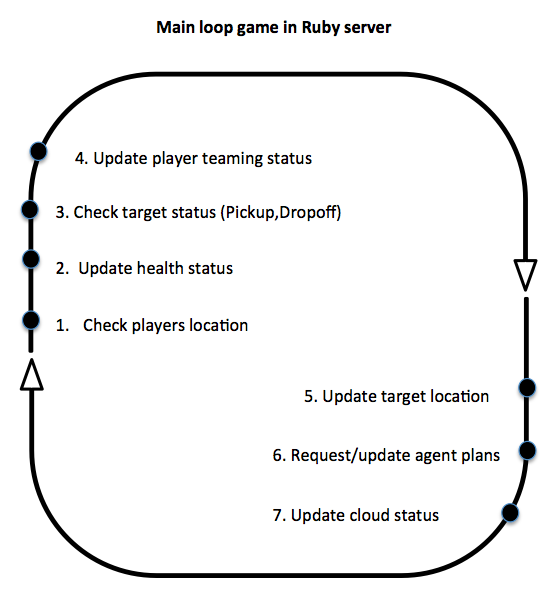
\includegraphics[width=1\textwidth]{img/Appendix/Mainloop}
  \caption{Handling of Game logic in Ruby server}
\end{figure}

\section{Data model}
\begin{table}[H]
\centering
\footnotesize
\begin{tabular}{llll}
\hline
{\bf Models}                        & {\bf Properties}                                                                                                                                                                                                       & {\bf Associations}                                                                                                                                  & {\bf Descriptions}                                                                                                               \\ \hline
\multicolumn{1}{|l|}{Game}         & \multicolumn{1}{l|}{\begin{tabular}[c]{@{}l@{}}id: {[}number{]}\\ update\_interval: {[}float{]}\\ grid\_size: {[}number{]}\\ simulation\_file: {[}string{]}\\ terrain: {[}string{]}\end{tabular}}                      & \multicolumn{1}{l|}{\begin{tabular}[c]{@{}l@{}}has\_many: targets\\ has\_many: players\\ has\_many: dropOffPoints\\ has\_many: plans\end{tabular}} & \multicolumn{1}{l|}{\begin{tabular}[c]{@{}l@{}}Represent config \\ information \\ of a particular \\ game session\end{tabular}} \\ \hline
\multicolumn{1}{|l|}{Player}       & \multicolumn{1}{l|}{\begin{tabular}[c]{@{}l@{}}id: {[}number{]}\\ latitude: {[}float{]}\\ longitude: {[}float{]}\\ role: {[}number{]}\\ initial: {[}string{]}\\ name: {[}string{]}\\ group: {[}string{]}\end{tabular}} & \multicolumn{1}{l|}{belongs\_to: game}                                                                                                             & \multicolumn{1}{l|}{\begin{tabular}[c]{@{}l@{}}Represent players \\ in the game\end{tabular}}                                   \\ \hline
\multicolumn{1}{|l|}{Task}         & \multicolumn{1}{l|}{\begin{tabular}[c]{@{}l@{}}id: {[}number{]}\\ latitude: {[}float{]}\\ longitude: {[}float{]}\\ type: {[}number{]}\\ status: {[}number{]}\end{tabular}}                                             & \multicolumn{1}{l|}{belongs\_to: game}                                                                                                             & \multicolumn{1}{l|}{\begin{tabular}[c]{@{}l@{}}Represent virtual\\ targets in the game\end{tabular}}                            \\ \hline
\multicolumn{1}{|l|}{DropOffPoint} & \multicolumn{1}{l|}{\begin{tabular}[c]{@{}l@{}}id: {[}number{]}\\ latitude: {[}float{]}\\ longitude: {[}float{]}\\ radius: {[}number{]}\end{tabular}}                                                                  & \multicolumn{1}{l|}{belongs\_to: game}                                                                                                             & \multicolumn{1}{l|}{\begin{tabular}[c]{@{}l@{}}Represent drop off\\ zone\end{tabular}}                                          \\ \hline
\multicolumn{1}{|l|}{Plan}         & \multicolumn{1}{l|}{id: {[}number{]}}                                                                                                                                                                                  & \multicolumn{1}{l|}{belongs\_to: game}                                                                                                             & \multicolumn{1}{l|}{\begin{tabular}[c]{@{}l@{}}Represent a plan \\ from agent\end{tabular}}                                     \\ \hline
\multicolumn{1}{|l|}{Frame}        & \multicolumn{1}{l|}{id: {[}number{]}}                                                                                                                                                                                  & \multicolumn{1}{l|}{belongs\_to: plan}                                                                                                             & \multicolumn{1}{l|}{\begin{tabular}[c]{@{}l@{}}Represent one \\ particular stage\\ in one frame\end{tabular}}                   \\ \hline
\multicolumn{1}{|l|}{Instruction}  & \multicolumn{1}{l|}{\begin{tabular}[c]{@{}l@{}}id: {[}number{]}\\ group: {[}string{]}\\ player: {[}number{]}\\ target: {[}number{]}\\ status: {[}number{]}\end{tabular}}                                               & \multicolumn{1}{l|}{belongs\_to: frame}                                                                                                            & \multicolumn{1}{l|}{\begin{tabular}[c]{@{}l@{}}Represent one \\ instruction sent to\\ one player\end{tabular}}                  \\ \hline
\end{tabular}
\caption{AtomicOrchid DB model}
\end{table}



\section{Agent-server protocol}
\begin{table}[H]
\centering
\tiny

\begin{tabular}{|l|l|l|l|}
\hline
{\bf Agent server interface}                                                    & {\bf Path}                                                                           & {\bf Parameters}                                                                                                                                                                                                                                                                                                                       & {\bf Return}                                                                                                                                           \\ \hline
Agent intialisation                                                             & \begin{tabular}[c]{@{}l@{}}/init\_session.php?\\ data=\{JSON\\ string\}\end{tabular} & \begin{tabular}[c]{@{}l@{}}\{\\    terrain: {[}string{]},\\    session\_id: {[}number{]},\\    targets: {[}array of targets{]},\\    dropoffzones:\\    {[}array of dropoff zones{]}\\ \}\end{tabular}                                                                                                                                 & \begin{tabular}[c]{@{}l@{}}\{\\   status:{[}ok|error{]}\\ \}\end{tabular}                                                                              \\ \hline
Check status                                                                    & \begin{tabular}[c]{@{}l@{}}/check\_status?\\ session\_id={[}number{]}\end{tabular}   & \begin{tabular}[c]{@{}l@{}}a number\\ representing game id\end{tabular}                                                                                                                                                                                                                                                                & \begin{tabular}[c]{@{}l@{}}\{\\    status: {[}inprogress|error|done{]}\\ \}\end{tabular}                                                               \\ \hline
\begin{tabular}[c]{@{}l@{}}Update target location\\ (study 2 only)\end{tabular} & \begin{tabular}[c]{@{}l@{}}/update\_target?\\ data=\{JSON\\ string\}\end{tabular}    & \begin{tabular}[c]{@{}l@{}}\{\\    session\_id: number,\\    targets:{[}array of targets{]}\\ \}\end{tabular}                                                                                                                                                                                                                          & \begin{tabular}[c]{@{}l@{}}\{\\   status: {[}ok|error{]}\\ \}\end{tabular}                                                                             \\ \hline
Fetch plan                                                                      & \begin{tabular}[c]{@{}l@{}}/fetch\_plan?\\ data=\{JSON\\ string\}\end{tabular}       & \begin{tabular}[c]{@{}l@{}}\{\\   session\_id: {[}number{]},\\   frame: {[}time frame{]},\\   rejections: {[}instructions rejected{]},\\   (study 2 only)\\   keep: {[}instructions to keep{]},\\   (study 3 only)\\   state: \{\\     players: {[}array of players{]},\\     targets: {[}array of targets{]}\\   \}\\ \}\end{tabular} & \begin{tabular}[c]{@{}l@{}}\{\\     plan: {[}\\       {[}array of instructions{]},\\       {[}array of instructions{]}\\    .... {]}\\ \}\end{tabular} \\ \hline
\end{tabular}
\caption{Agent server protocol}
\end{table}


\chapter{Appendix to study 1}
\section{Game area and set-up}

\begin{figure}[H]
  \centering
  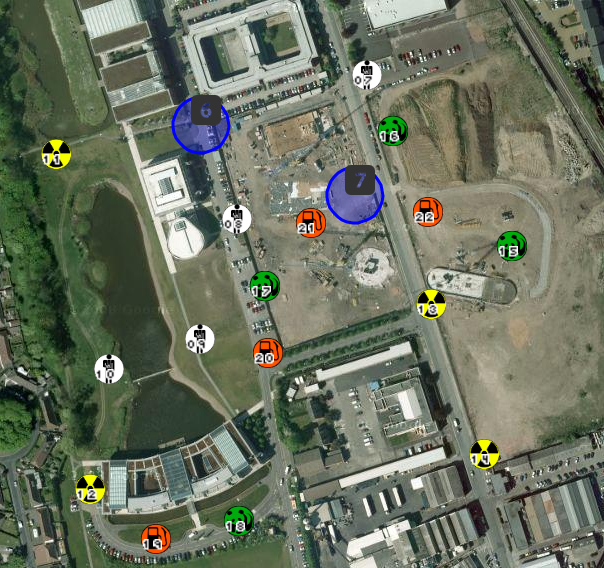
\includegraphics[width=1\textwidth]{img/Appendix/targets1}
  \caption{Target distribution in study 1}
\end{figure}


\section{Participant demographic}

\begin{table}[H]
\centering
\footnotesize
\rotatebox{90}{
\begin{tabular}{|l|l|l|l|l|l|l|l|}
\hline
Initials & Gender & Occupation & \begin{tabular}[c]{@{}l@{}}Mobile OS \\ experience\end{tabular} & \begin{tabular}[c]{@{}l@{}}Location game \\ experence\end{tabular} & \begin{tabular}[c]{@{}l@{}}Navigation app\\  experience\end{tabular} & \begin{tabular}[c]{@{}l@{}}Map reading\\  skill\end{tabular} & \begin{tabular}[c]{@{}l@{}}Know other \\ participants\end{tabular} \\ \hline
NH       & M      & Student    & Android                                                         & YES                                                                & YES                                                                  & MEDIUM                                                       &                         \\ \hline
RL       & M      & Student    & iOS                                                             & NO                                                                 & YES                                                                  & HIGH                                                         &                         \\ \hline
JP       & F      & Student    & Android, Wndows                                                 & NO                                                                 & YES                                                                  & HIGH                                                         & TD                      \\ \hline
TD       & M      & Student    & iOS                                                             & NO                                                                 & YES                                                                  & MEDIUM                                                       & JP                      \\ \hline
TV       & M      & Student    & Android                                                         & NO                                                                 & YES                                                                  & HIGH                                                         &                         \\ \hline
HQ1      & M      & Student    & iOS, Blackberry                                                 & NO                                                                 & YES                                                                  & MEDIUM                                                       &                         \\ \hline
HQ2      & M      & Researcher & iOS                                                             & NO                                                                 & YES                                                                  & HIGH                                                         &                         \\ \hline
\end{tabular}}
\caption{Participants in session A, Study 1}
\end{table}



\begin{table}[H]
\centering
\footnotesize
\rotatebox{90}{
\begin{tabular}{|l|l|l|l|l|l|l|l|}
\hline
Initials & Gender & Occupation & \begin{tabular}[c]{@{}l@{}}Mobile OS \\ experience\end{tabular} & \begin{tabular}[c]{@{}l@{}}Location game \\ experence\end{tabular} & \begin{tabular}[c]{@{}l@{}}Navigation app\\  experience\end{tabular} & \begin{tabular}[c]{@{}l@{}}Map reading\\  skill\end{tabular} & \begin{tabular}[c]{@{}l@{}}Know other \\ participants\end{tabular} \\ \hline
D2       & M      & Student    & Android,Windows                                                 & NO                                                                 & YES                                                                  & MEDIUM                                                       &                                                                    \\ \hline
D1       & M      & Student    & Android                                                         & NO                                                                 & YES                                                                  & HIGH                                                         &                                                                    \\ \hline
BR       & F      & Student    & iOS                                                             & NO                                                                 & YES                                                                  &                                                              & KL,HQ1                                                             \\ \hline
KL       & F      & Student    & iOS                                                             & NO                                                                 & NO                                                                   & HIGH                                                         & BR,HQ1                                                             \\ \hline
KY       & F      & Student    & Android,Windows                                                 & NO                                                                 & NO                                                                   & MEDIUM                                                       &                                                                    \\ \hline
JH       & M      & Student    & Android,iOS                                                     & NO                                                                 & YES                                                                  & HIGH                                                         &                                                                    \\ \hline
HD       & F      & Student    & No experience                                                   & NO                                                                 & NO                                                                   & MEDIUM                                                       &                                                                    \\ \hline
MF       & M      & Researcher & iOS                                                             & NO                                                                 & NO                                                                   & HIGH                                                         &                                                                    \\ \hline
HQ1      & F      & Student    & iOS                                                             & NO                                                                 & YES                                                                  &                                                              &                                                                    \\ \hline
HQ2      & F      & Student    & iOS                                                             & NO                                                                 & YES                                                                  &                                                              & HD                                                                 \\ \hline
HQ3      & F      & Student    & iOS                                                             & NO                                                                 & YES                                                                  &                                                              & KL,BR                                                              \\ \hline
\end{tabular}}
\caption{Participants in Session B, Study 1}
\end{table}



\section{Game event visualisation}
\begin{figure}[H]
  \centering
  \rotatebox{90}{
  	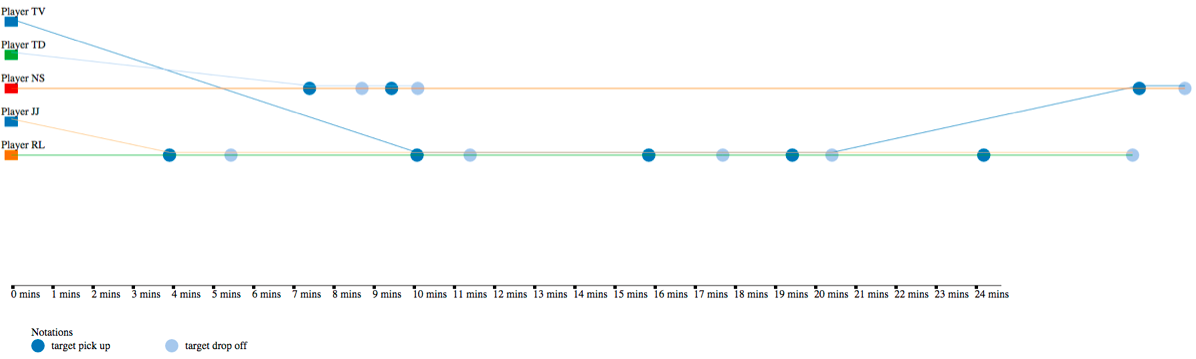
\includegraphics[width=1.8\textwidth]{img/Appendix/study1A}
  }
  \caption{Event visualisation of Study 1, Session A}
  
\end{figure}

\section{Game event visualisation}
\begin{figure}[H]
  \centering
  \rotatebox{90}{
  	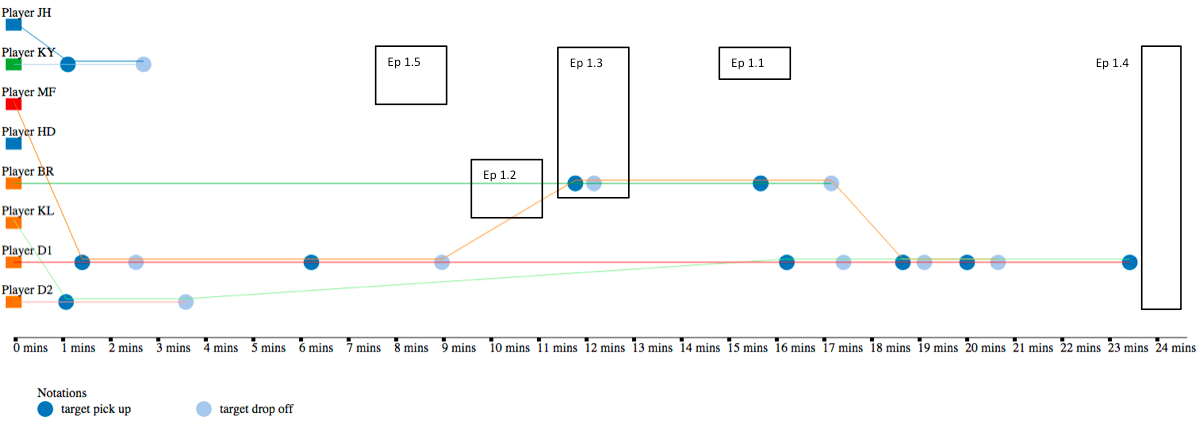
\includegraphics[width=1.8\textwidth]{img/Appendix/study1B}
  }
  \caption{Event visualisation of Study 1, Session B}
 
\end{figure}



\chapter{Appendix to study 2}



\section{Game area and set-up}
\begin{figure}[H]
  \centering
  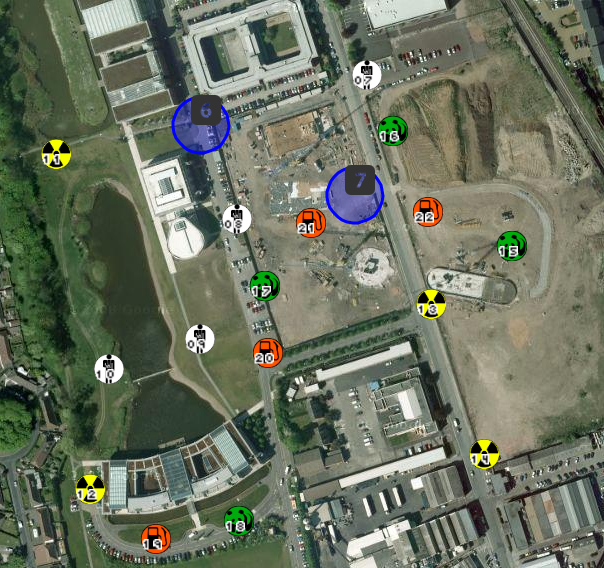
\includegraphics[width=1\textwidth]{img/Appendix/targets1}
  \caption{Target distribution in study 2}
\end{figure}

\section{Participant demographic}
\begin{table}[H]
\centering
\footnotesize
\rotatebox{90}{
\begin{tabular}{|l|l|l|l|l|l|l|l|l|}
\hline
Initials & Age & Gender & Occupation      & \begin{tabular}[c]{@{}l@{}}Mobile OS \\ experience\end{tabular} & \begin{tabular}[c]{@{}l@{}}Location game \\ experence\end{tabular} & \begin{tabular}[c]{@{}l@{}}Navigation app\\  experience\end{tabular} & \begin{tabular}[c]{@{}l@{}}Map reading\\  skill\end{tabular} & \begin{tabular}[c]{@{}l@{}}Know other \\ participants\end{tabular} \\ \hline
AC       & 26  & M      & Student         & iOS                                                             & YES                                                                & YES                                                                  & MEDIUM                                                       &                                                                    \\ \hline
HB       & 19  & F      & Student         & iOS                                                             & NO                                                                 & YES                                                                  & MEDIUM                                                       & KD                                                                 \\ \hline
AR       & 18  & M      & Student         & iOS,Android                                                     & YES                                                                & YES                                                                  & HIGH                                                         &                                                                    \\ \hline
AW       & 18  & M      & Student         & Android                                                         & NO                                                                 & NO                                                                   & MEDIUM                                                       &                                                                    \\ \hline
LC       & 27  & M      & Event organiser & Nodia                                                           & NO                                                                 & NO                                                                   & HIGH                                                         &                                                                    \\ \hline
YF       & 24  & F      & Student         & Android                                                         & YES                                                                & YES                                                                  & HIGH                                                         &                                                                    \\ \hline
DD       & 32  & F      & Student         & iOS                                                             & NO                                                                 & YES                                                                  & HIGH                                                         &                                                                    \\ \hline
KD       & 20  & M      & Student         & Android                                                         & YES                                                                & YES                                                                  & HIGH                                                         &                                                                    \\ \hline
HQ       & 24  & M      & Student         & Android                                                         & NO                                                                 & NO                                                                   & MEDIUM                                                       &                                                                    \\ \hline
\end{tabular}}
\caption{Participants in Session A, Study 2}
\end{table}

\begin{table}[H]
\centering
\footnotesize
\rotatebox{90}{
\begin{tabular}{|l|l|l|l|l|l|l|l|l|}
\hline
Initials & Age & Gender & Occupation & \begin{tabular}[c]{@{}l@{}}Mobile OS \\ experience\end{tabular} & \begin{tabular}[c]{@{}l@{}}Location game \\ experence\end{tabular} & \begin{tabular}[c]{@{}l@{}}Navigation app\\  experience\end{tabular} & \begin{tabular}[c]{@{}l@{}}Map reading\\  skill\end{tabular} & \begin{tabular}[c]{@{}l@{}}Know other \\ participants\end{tabular} \\ \hline
DP       & 26  & M      & Student    & iOS                                                             & NO                                                                 & YES                                                                  & MEDIUM                                                       &                                                                    \\ \hline
LT       & 19  & F      & Student    & iOS                                                             & NO                                                                 & YES                                                                  & HIGH                                                         & NK,NW                                                              \\ \hline
CR       & 18  & M      & Student    & iOS,Android                                                     & NO                                                                 & YES                                                                  & HIGH                                                         &                                                                    \\ \hline
SS       & 18  & M      & Student    & Android                                                         & NO                                                                 & YES                                                                  & HIGH                                                         & PC                                                                 \\ \hline
NK       & 27  & F      & Student    & iOS                                                             & NO                                                                 & YES                                                                  & MEDIUM                                                       & LT,NW                                                              \\ \hline
NW       & 24  & F      & Student    & iOS                                                             & NO                                                                 & YES                                                                  & MEDIUM                                                       & NK,LT                                                              \\ \hline
JL       & 32  & F      & Student    & no experience                                                   & NO                                                                 & YES                                                                  & HIGH                                                         &                                                                    \\ \hline
PC       & 20  & F      & Student    & iOS                                                             & NO                                                                 & YES                                                                  & MEDIUM                                                       & SS                                                                 \\ \hline
HQ       & 24  & M      & Student    & iOS                                                             & NO                                                                 & YES                                                                  & MEDIUM                                                       &                                                                    \\ \hline
\end{tabular}}
\caption{Participants in Session B, Study 2}
\end{table}


\section{Game event visualisation}
\begin{figure}[H]
  \centering
  \rotatebox{90}{
  	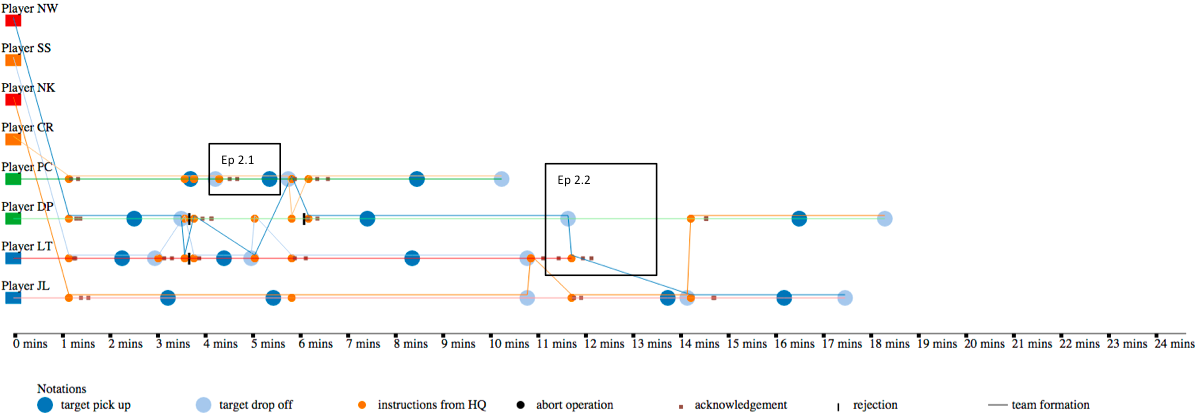
\includegraphics[width=1.8\textwidth]{img/Appendix/study2A}
  }
  \caption{Event visualisation of Study 2, Session A}
  
\end{figure}

\section{Game event visualisation}
\begin{figure}[H]
  \centering
  \rotatebox{90}{
  	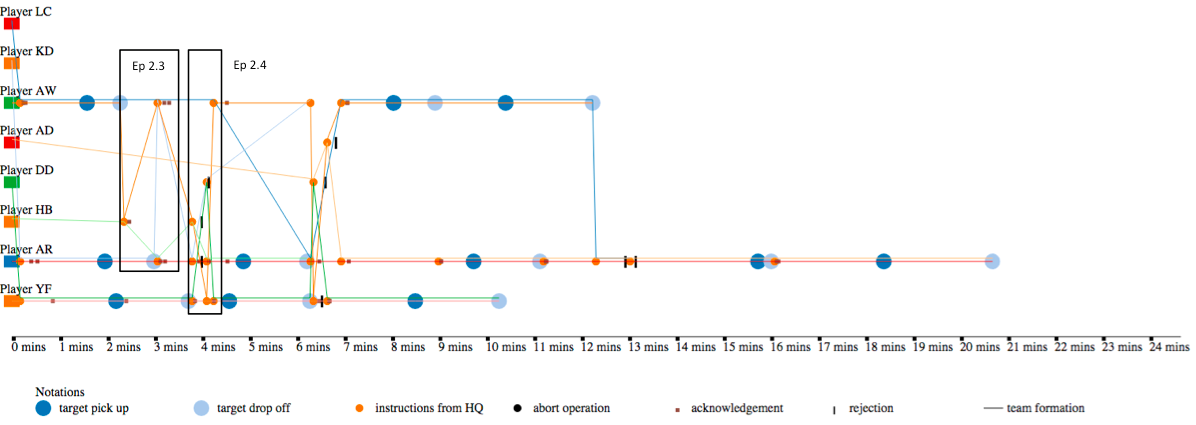
\includegraphics[width=1.8\textwidth]{img/Appendix/study2B}
  }
  \caption{Event visualisation of Study 2, Session B}
 
\end{figure}

\chapter{Appendix to study 3}

\section{Game area and set-up}
\begin{figure}[H]
  \centering
  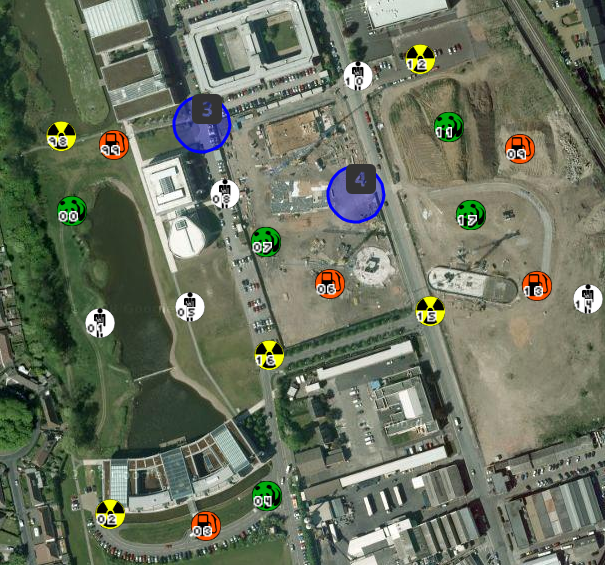
\includegraphics[width=1\textwidth]{img/Appendix/targets2}
  \caption{Target distribution in study 3}
\end{figure}


\section{Participant demographic}
\begin{table}[H]
\centering
\rotatebox{90}{
\begin{tabular}{|l|l|l|l|l|l|l|l|l|}
\hline
Initials & Age & Gender     & Occupation & \begin{tabular}[c]{@{}l@{}}Mobile OS\\ experience\end{tabular} & \begin{tabular}[c]{@{}l@{}}Location game\\ experience\end{tabular} & \begin{tabular}[c]{@{}l@{}}Navigation app\\ experience\end{tabular} & \begin{tabular}[c]{@{}l@{}}Map reading\\ skill\end{tabular} & \begin{tabular}[c]{@{}l@{}}Know other\\ participants\end{tabular} \\ \hline
WX       & 25  & student    & F          & Android                                                        & NO                                                                 & YES                                                                 & MEDUIM                                                      & BW                                                                \\ \hline
LR       & 23  & student    & M          & Android,iOS                                                    & YES                                                                & YES                                                                 & MEDUIM                                                      &                                                                   \\ \hline
NG       & 26  & student    & M          & Android,iOS                                                    & YES                                                                & NO                                                                  & HIGH                                                        &                                                                   \\ \hline
MV       & 22  & student    & M          & iOS                                                            & NO                                                                 & YES                                                                 & HIGH                                                        &                                                                   \\ \hline
DI       & 26  & researcher & M          & Android                                                        & YES                                                                & YES                                                                 & HIGH                                                        &                                                                   \\ \hline
BW       & 23  & student    & M          & Windows                                                        & NO                                                                 & YES                                                                 & MEDUIM                                                      & XW                                                                \\ \hline
LT       & 23  & student    & F          & iOS                                                            & NO                                                                 & YES                                                                 & MEDUIM                                                      & DI                                                                \\ \hline
YI       & 23  & student    & M          & iOS                                                            & NO                                                                 & YES                                                                 & MEDUIM                                                      &                                                                   \\ \hline
HQ1      & 25  & student    & M          & iOS                                                            & YES                                                                & YES                                                                 & MEDUIM                                                      & HQ2                                                               \\ \hline
HQ2      & 24  & student    & M          & iOS                                                            & YES                                                                & YES                                                                 & MEDUIM                                                      & HQ1                                                               \\ \hline
\end{tabular}}
\caption{Participants in Session A, Study 3}
\end{table}



\begin{table}[H]
\centering
\rotatebox{90}{
\begin{tabular}{|l|l|l|l|l|l|l|l|l|}
\hline
Initials & Age & Gender     & Occupation & \begin{tabular}[c]{@{}l@{}}Mobile OS\\ experience\end{tabular} & \begin{tabular}[c]{@{}l@{}}Location game\\ experience\end{tabular} & \begin{tabular}[c]{@{}l@{}}Navigation app\\ experience\end{tabular} & \begin{tabular}[c]{@{}l@{}}Map reading\\ skill\end{tabular} & \begin{tabular}[c]{@{}l@{}}Know other\\ participants\end{tabular} \\ \hline
GS       & 29  & student    & M          & Android                                                        & NO                                                                 & YES                                                                 & MEDUIM                                                      & BW                                                                \\ \hline
WB       & 25  & student    & F          & Android                                                        & NO                                                                 & YES                                                                 & HIGH                                                        &                                                                   \\ \hline
CE       & 24  & student    & F          & Android, Windows, iOS                                          & NO                                                                 & YES                                                                 & MEDUIM                                                      &                                                                   \\ \hline
DS       & 24  & student    & M          & Android                                                        & YES                                                                & NO                                                                  & MEDUIM                                                      &                                                                   \\ \hline
MP       & 24  & researcher & M          & Android, iOS                                                   & YES                                                                & YES                                                                 & MEDUIM                                                      &                                                                   \\ \hline
MB       & 25  & student    & M          & Android                                                        & NO                                                                 & NO                                                                  & HIGH                                                        & CY,WB,HQ1,HQ2                                                     \\ \hline
DS       & 25  & student    & M          & Android                                                        & NO                                                                 & YES                                                                 & MEDUIM                                                      & DS                                                                \\ \hline
CY       & 25  & student    & M          & iOS                                                            & YES                                                                & YES                                                                 & MEDUIM                                                      & MB                                                                \\ \hline
HQ1      & 34  & student    & M          & Android                                                        & YES                                                                & YES                                                                 & MEDUIM                                                      & HQ2,MP                                                            \\ \hline
HQ2      & 32  & student    & M          & Android                                                        & YES                                                                & YES                                                                 & MEDUIM                                                      & HQ1,MP                                                            \\ \hline
\end{tabular}}
\caption{Participants in Session B, Study 3}
\end{table}
\section{Game event visualisation}
\begin{figure}[H]
  \centering
  \rotatebox{90}{
  	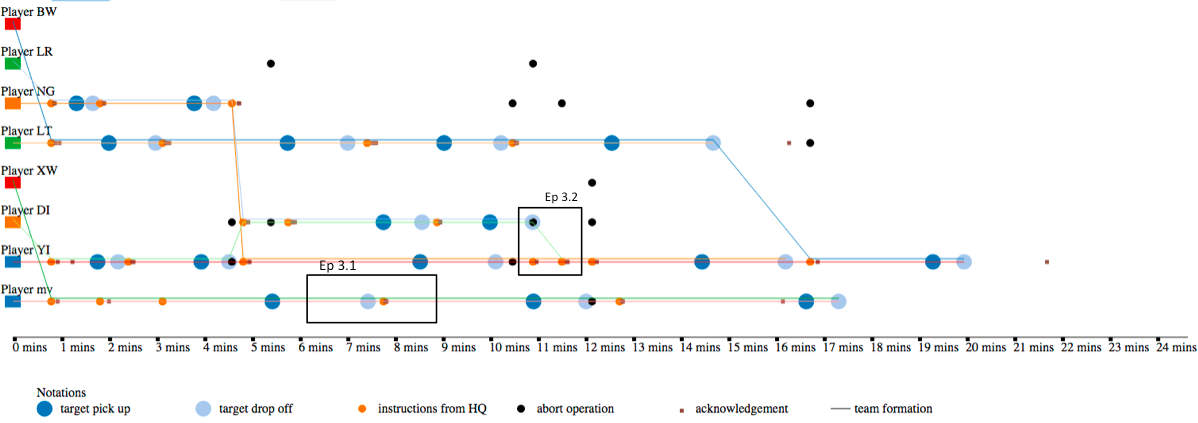
\includegraphics[width=1.8\textwidth]{img/Appendix/study3A}
  }
  \caption{Event visualisation of Study 3, Session A}
\end{figure}

\section{Game event visualisation}
\begin{figure}[H]
  \centering
  \rotatebox{90}{
  	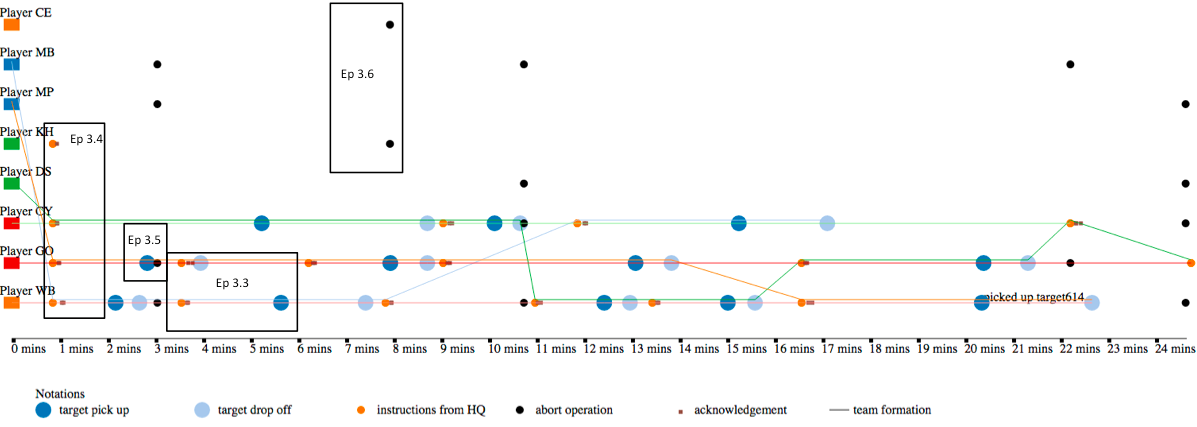
\includegraphics[width=1.8\textwidth]{img/Appendix/study3B}
  }
  \caption{Event visualisation of Study 3, Session B}
\end{figure}